% Especificaciones del tamaño de letra, tamaño de hoja, márgenes, librerias, etc.
\documentclass[letterpaper]{article}
\usepackage[english]{babel}
\usepackage[utf8]{inputenc}
\usepackage[T1]{fontenc}
\usepackage{mathrsfs}
\usepackage{amsmath}
\usepackage{graphicx}
\usepackage[justification=centering]{caption}
\usepackage{subcaption}
\usepackage[hidelinks]{hyperref}
\usepackage{url}
\usepackage{amssymb}
\usepackage{float}
\usepackage[framed, numbered]{matlab-prettifier}
\usepackage{lipsum}
\usepackage{multicol}
\usepackage{fancyhdr}
%\usepackage[framed, numbered, autolinebreaks, useliterate]{mcode}
\usepackage[margin=1in]{geometry}
\renewcommand{\baselinestretch}{1.5}

\pagestyle{fancy}
\fancyhf{}
\rhead{C. A. Vásquez}
\lhead{Formación de Cristales}
\rfoot{\thepage}

% Enlace Bibliografía
\usepackage{csquotes}
\usepackage[backend=biber, sorting=none]{biblatex}
\addbibresource{referencias.bib}

% Titulo, autores, fecha.
\title{\textbf{Formación de Cristales}}
\author{C. A. Vásquez\\
\footnotesize {\textit{UABC, Ingeniería Aeroespacial, Mexicali, México}}\\
\footnotesize \texttt{a1155057@uabc.edu.mx}}
\date{}
% Inicio del documento
\begin{document}
\maketitle

\section*{Introducción}
Un sólido cristalino puede pensarse como un arreglo periódico de un grupo representativo de átomos, moléculas o iones. Esto nos permite construir un cristal mediante una estructura mínima llamada celda unitaria, que trasladamos por el espacio.

La importancia tecnológica de los sólidos cristalinos está en relación con sus propiedades eléctricas, ópticas o magnéticas que son distintivas de las estructuras periódicas y en base a las cuales se fabrican muchos dispositivos de la vida actual: láseres, LEDs, fotómetros, celdas solares, transistores, pantallas de TV, etc. Todas estas propiedades están relacionadas con la estructura del material y con la distribución de los electrones de valencia de los átomos que forman parte del cristal. \supercite{aldebe19}
\section*{Disoluciones}
\begin{enumerate}
	\item ¿Qué son las disoluciones? 

		Es una mezcla homogénea de dos o más sustancias.

	\item ¿De qué depende la facilidad de disolución de un soluto en un disolvente?

		La facilidad con la que una partícula de soluto reemplaza a una molécula de disolvente depende de la fuerza relativa de tres tipos de interacciones:
		\begin{itemize}
			\item interacción disolvente-disolvente
			\item interacción soluto-soluto
			\item interacción disolvente-soluto
		\end{itemize}

	\item Distinga entre una disolución no saturada, saturada y sobresaturada.

		\textbf{Disolución saturada:} contiene la máxima cantidad de un soluto que se disuelve en un disolvente en particular, a una temperatura específica.

		\textbf{Disolución no saturada:} contiene menor cantidad de soluto que la que es capaz de disolver.

		\textbf{Disolución sobresaturada:} contiene más soluto que el que puede haber en una disolución saturada.
		
	\item ¿A partir de qué tipo de disolución puede ocurrir cristalización o precipitación? ¿Cuál es la diferencia entre un cristal y un precipitado?

		Con el tiempo, las disoluciones sobresaturadas forman cristales debido a que el soluto se separa de la disolución en forma de cristales.

		La cristalización es el proceso en el cual el soluto disuelto se separa de la disolución y forma cristales. Tanto la precipitación como la cristalización describen la separación de un exceso de la solución sólida a partir de la disolución sobresaturada. Sin embargo, los sólidos que se forman durante estos dos procesos tienen apariencia diferente. En general, pensamos que los precipitados están formados por partículas pequeñas, en tanto que los cristales pueden ser grandes y bien formados.

	\item Describir brevemente el proceso de disolución a nivel molecular. Utilice como ejemplo la disolución de un sólido en un líquido.

		Cuando una sustancia (el soluto) se disuelve en otra (el disolvente), las partículas del soluto se dispersan en el disolvente. Las partículas de soluto ocupan lugares que estaban ocupados por las moléculas de disolvente. La facilidad con la que una partícula de soluto reemplaza a una molécula de disolvente depende de la fuerza relativa de tres tipos de interacciones:

	\item ¿Qué es la solvatación y qué factores influyen en el grado de solvatación?
		
		Es el proceso mediante el cual un ión o una molécula se rodea por moléculas del disolvente, distribuidas de una forma específica. Cuando el disolvente es agua, este proceso se llama hidratación.

		Depende de la naturaleza de las moléculas, en especial si tienen o no un momento dipolar, su carga, etc.

	\item Describir los factores que afectan la solubilidad de un sólido en un líquido.

		El primer factor es energético, que determina si un proceso de disolución es exotérmico o endotérmico. El segundo factor se refiere a la tendencia hacia el desorden inherente a todos los procesos naturales. Cuando se mezclan las moléculas de soluto y de disolvente para formar una disolución hay un incremento de aleatoriedad o desorden,

	\item ¿Qué significa decir que dos líquidos son miscibles?

		Se dice que dos líquidos son miscibles si son completamente solubles entre sí en todas proporciones.

	\item Describa el proceso de cristalización fraccionada y su aplicación.
	
		Es la separación de una mezcla de sustancias en sus componentes puros con base en sus diferentes solubilidades. Una de las aplicaciones son, al momento de tener una sustancia contaminada, la posibilidad de que la disolución cuente con distintas propiedades a distintas temperaturas brinda la posibilidad de separarlas mediante este método. Es posible separar un compuesto de la disolución, manteniendo el o los otros solutos disueltos. Posteriormente se pueden separar mediante un proceso de filtración.

\end{enumerate}

*Respuestas obtenidas del libro \textit{Química} de Raymond Chang.\supercite{chang13}
\section*{Formación de Cristales}
El proceso de formación de cristales es muy sencillo, sin embargo, dependiendo de la sustancia, podría tomar algo de tiempo. Hay muchos factores que se involucran, pero los más importantes son la solucióin que se prepara y el medio en el que se deja reposar la solución.

Considerando estas variantes, la metodología utilizada fue la que recomendaba la Salt Association en su página web. \supercite{sa19} Los materiales utilizados son los siguientes:

\begin{itemize}
	\item Sal de mar (NaCl).
	\item Agua potable.
	\item Recipiente de cristal.
	\item Hilo.
	\item Lápiz.
\end{itemize}

Para que la formación de cristales sea óptima y nos aseguremos desde el inicio que se formará éste, es necesario que las sustancias que utilicemos sean lo más puras posibles. Es por esto que la sal utilizada es de mar. Si fuese sal yodizada entonces, por los elementos extra con los que cuenta hubiese sido más complicado obtener los cristales.

Lo mismo ocurre con el agua. Lo recomendado es utilizar agua destilada ya que nos asegura que no habrá otros elementos como cloro o sodio. A pesar de esto, si es imposible conseguir el agua destilada, agua potable también nos proporciona la posibilidad de que el cristal se forme, como fue el caso del cristal que mostraremos en las siguientes secciones.

El proceso para la preparación del material y su asentamiento se describe a continuación:

\begin{enumerate}
	\item Primeramente el agua potable con la que se contaba es puesta a hervir. Esto con el fin de facilitar la solventación de la sal en el disolvente.
	\item Después de haber hervido el agua, procedemos a añadir la sal. Es importante remarcar que la concentración de sal tiene que ser muy alta, tanto para crear una solución sobresaturada, ya que ésta es la que permite que se depositen cristales debido al exceso de soluto. Para llegar al punto de una solución sobresaturada es necesario disolver la sal en el agua hasta que ésta ya no pueda mezclarse más. En ese entonces sabremos que nuestra solución es sobresaturada.
	\item Posteriormente, una vez hecha nuestra mezcla sobresaturada de agua y sal, dejamos que el agua disminuya su temperatura a la ambiental y la trasladamos a un recipiente de cristal. Esto con el fin de evitar que el mismo recipiente reaccione con la disolución y evite la formación de cristales.
	\item Siguiente, a un lápiz atamos un pequeño hilo blanco, el cual se dejará reposar dentro de la disolución. Esto ayudará a la formación de cristales, actuándo como un centro de nucleación donde se podrán depositar más moléculas de cloruro de sodio.
	\item El último paso es esperar. Dependiendo de la concentración salina de la disolución, la formación del cristal puede tardar desde medio día hasta tres días.
\end{enumerate}

A continuación se muestran fotografías del equipo utilizado y su configuración:

\begin{figure}[H]
	\centering
	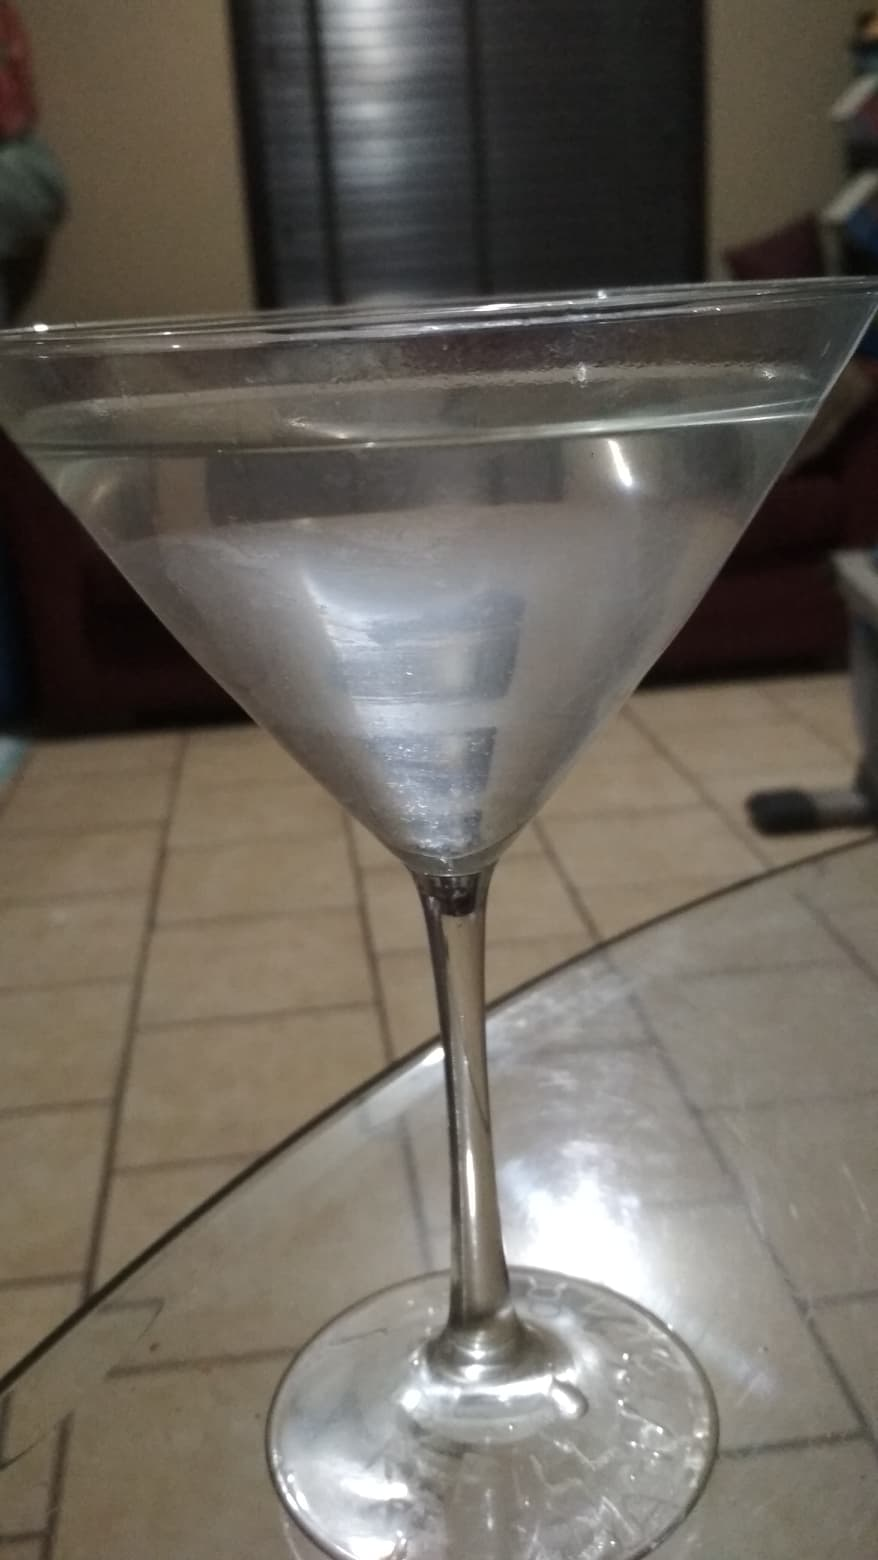
\includegraphics[width=0.7\textwidth]{1.jpg}
	\caption{Disolución en el recipiente de vidrio.}
\end{figure}

\begin{figure}[H]
	\centering
	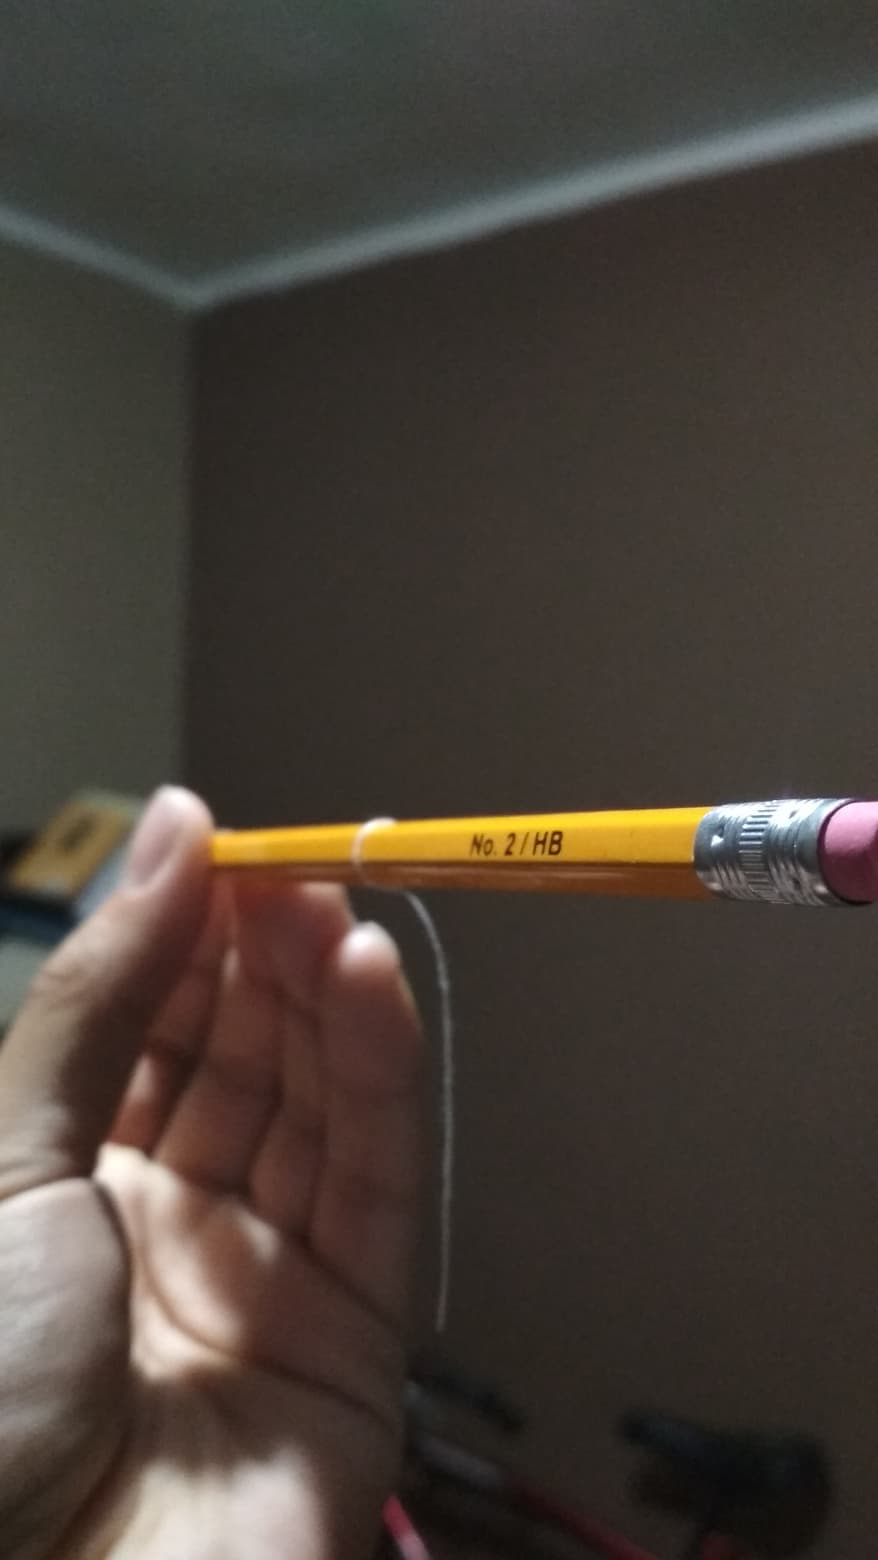
\includegraphics[width=0.7\textwidth]{2.jpg}
	\caption{Lápiz con un trozo de hilo atado a él.}
\end{figure}

\begin{figure}[H]
	\centering
	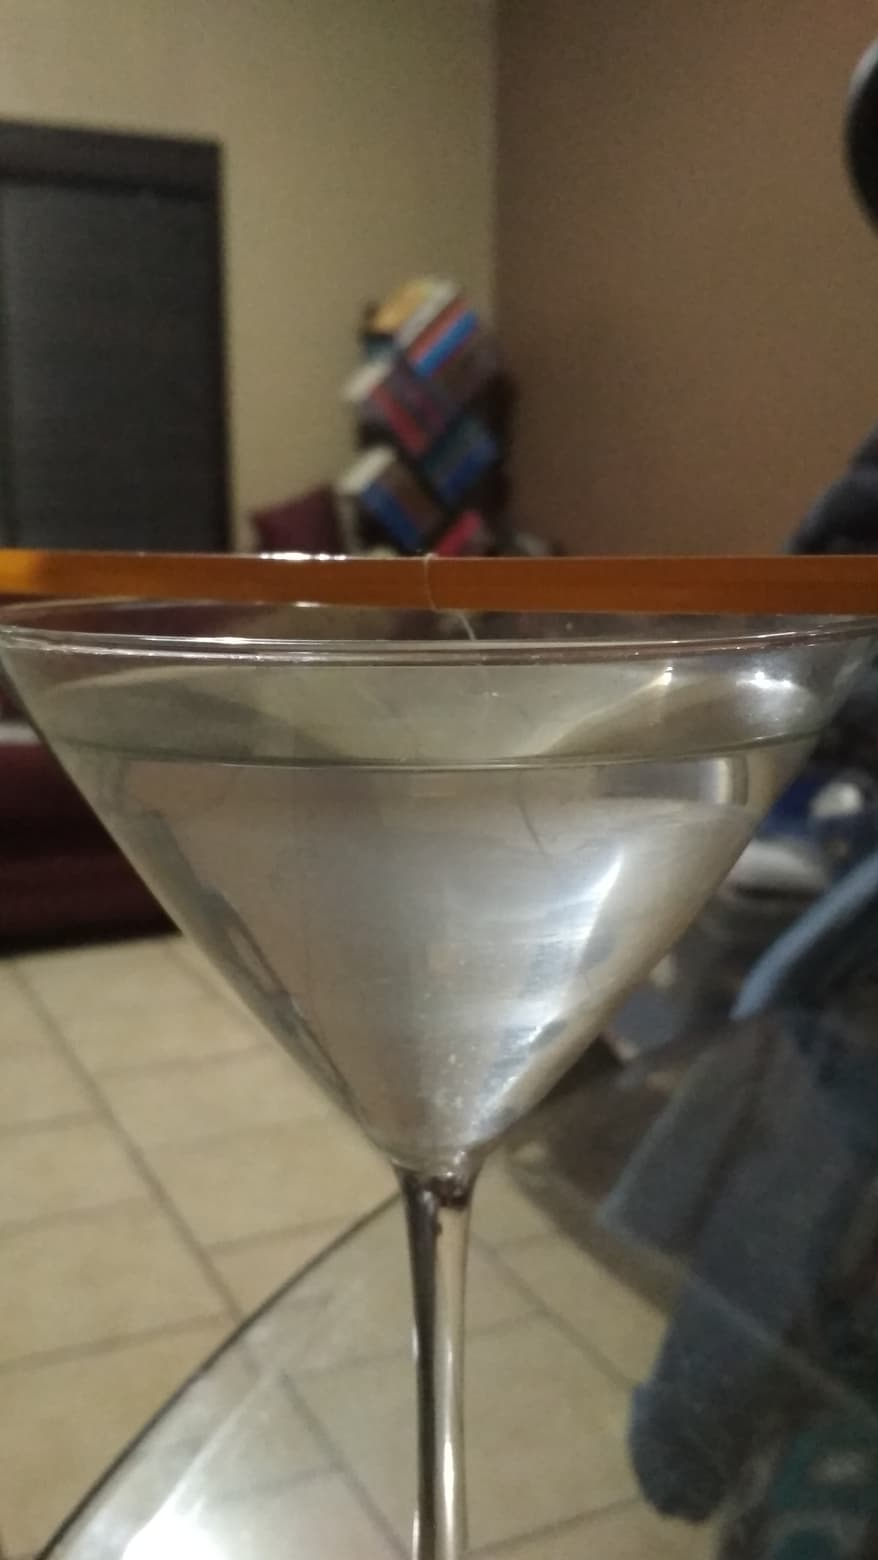
\includegraphics[width=0.7\textwidth]{3.jpg}
	\caption{Configuración de los materiales, nótese el hilo queda sumergido en la disolución para facilitar el depósito de cristales}
\end{figure}
\section*{Resultados}
Las siguientes imágenes muestran los resultados obtenidos después de haber esperado durante 3 días.

\begin{figure}[H]
	\centering
	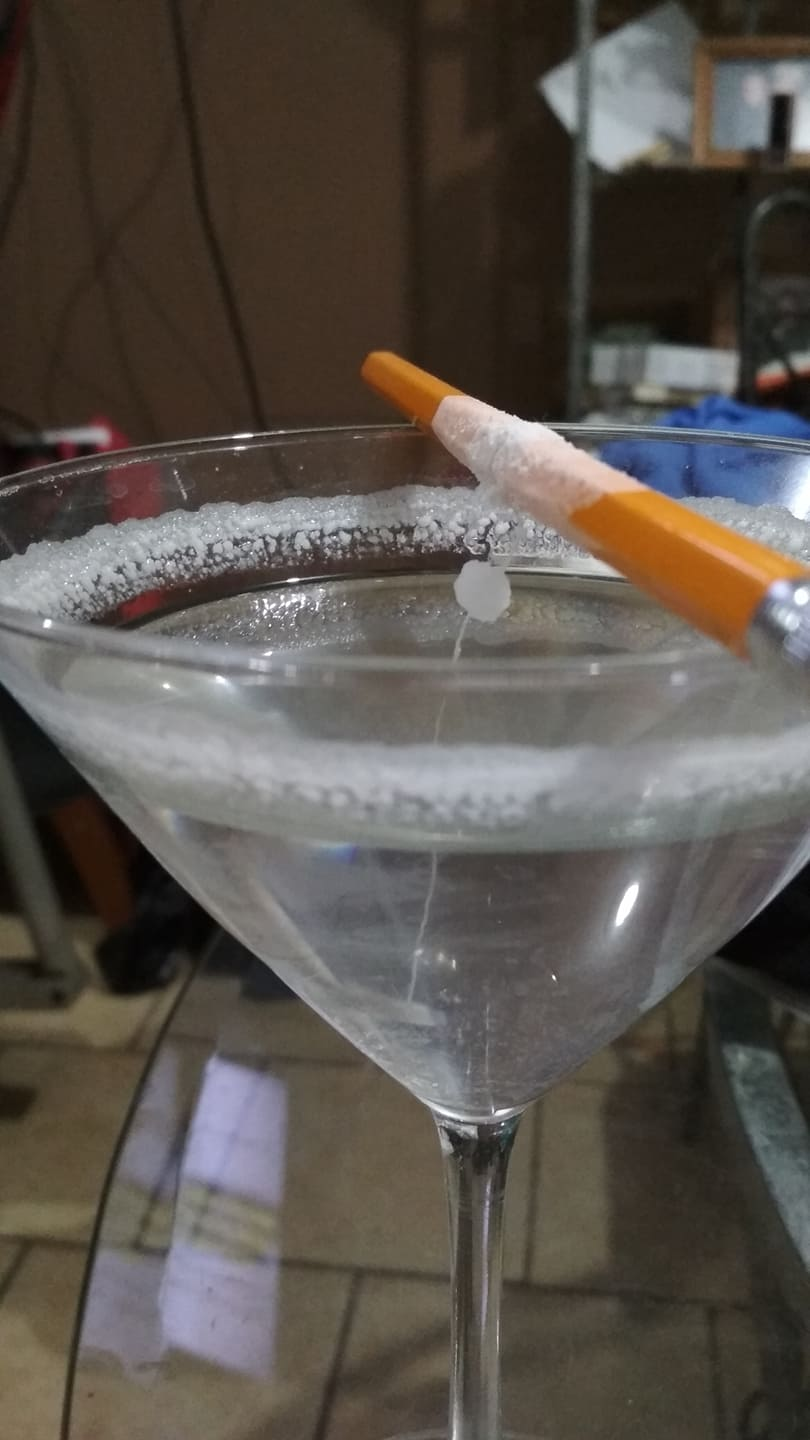
\includegraphics[width=0.65\textwidth]{4.jpg}
	\caption{Cristales depositados en la fase gaseosa de la disoluciön. La superficie del fluido, el hilo y el lápiz cubiertos de cristales de sal.}
\end{figure}

\begin{figure}[H]
	\centering
	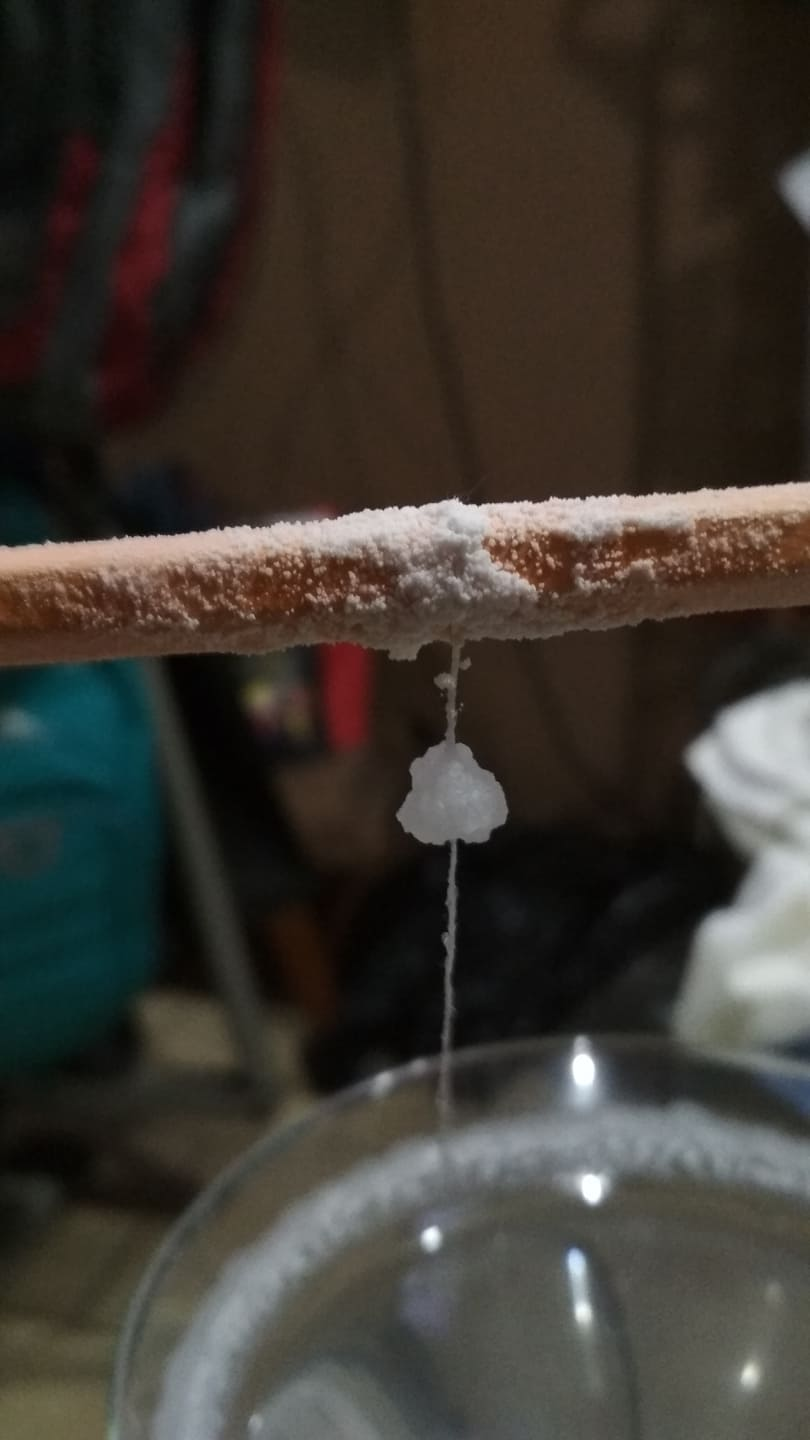
\includegraphics[width=0.7\textwidth]{5.jpg}
	\caption{Gran pedazo de cristal de sal colgando del hilo.}
\end{figure}


Como podemos observar, el cristal se formó satisfactoriamente a lo largo de la fase gaseosa de la disolución, en el hilo y en el lápiz.
\subsubsection*{Discusión de los Resultados}
El cristal se formó satisfactoriamente, pero es poco intuitivo el porqué los depósitos de cristales crecerían en el lápiz, el hilo sobre la superficie de la fase líquida y el borde del recipiente.

No existen pruebas rigurosas, pero es posible especular que la disolución no se encontraba sobresaturada y, debido a esto, a medida en que las moléculas de agua se evaporaban, éstas traían consigo moléculas de cloruro de sodio, y cuando se encontraban en grandes concentraciones en el hilo, el lápiz y la parte del recipiente de cristal, éstos se depositaban sin la necesidad de utilizar mucha energía.

Lo que sería necesario en próximas configuraciones del experimento es tener un método más cuantitativo para medir el nivel de saturación que existe en la disolución. El método cualitativo utilizado cuenta con mucha incertidumbre, así que puede que éstos nos haya orillado a tomar una decisión errónea al momento de dictaminar cuándo la solución se encontraba sobresaturada.

\section*{Conclusiones}

A pesar de haber obtenido los cristales mostrados anteriormente, es evidente que no fue como se predijo. Es posible que la misma naturaleza de la disolución no permita que los cristales se depositen y coexistan en el medio acuoso (fase líquida). Esto no es más que una oportunidad más para estudiar más a fondo el comportamiento verdadero de estas soluciones y cómo se realiza la formación de los cristales a escalas pequeñas hablando específicamente de el soluto y solvente utilizados en esta ocasión.

Con certeza podemos concluir que el cristal obtenido fue un policristal debido al arreglo poco ordenado que éste tiene. Los monocristales usualmente presentan formas geométricas mucho más regulares porque comienzan a crecer de un solo grano, pero en el caso de los cristales de sal, éstos se presentan con distintos puntos de nucleación, dando forma a un policristal.

Como pensamiento final, podemos decir que a pesar de haber analizado con anterioridad las posibilidades, es posible que incluso después de haber creído llegar a una conclusión puede que ésta sea errónea y los resultados sugieran otro tipo de explicación, lo cual da una área de oportunidad para la investigación y generación de nuevo conocimiento.
%%%%% Bib
\renewcommand\refname{Referencias}
\printbibliography

\end{document}
